\documentclass[11pt,a4paper]{article}
\usepackage[utf8]{inputenc}
\usepackage[margin=22mm]{geometry}
\usepackage{amsmath,amssymb}
\usepackage{booktabs}
\usepackage{graphicx}
\usepackage{tikz}
\usetikzlibrary{arrows.meta,positioning,calc}
\usepackage{pgfplots}
\pgfplotsset{compat=1.17}
\usepackage[hidelinks]{hyperref}
\usepackage{caption}
\captionsetup{font=small}

\newcommand{\Vdo}{V_{d0}}
\newcommand{\Id}{I_d}
\newcommand{\ex}{e_x}
\newcommand{\dx}{d_x}
\newcommand{\Ell}{E_{2}}

\title{Sizing of a 400\,V / 1\,MW thyristor AC/DC supply\\
\large for a 1100\,A resistive load at 16.4--200\,V with 5\,\% line-side THD$_i$}
\author{Davide Bagnara}
\date{September 2026}

\begin{document}
\maketitle

\begin{abstract}
This note sizes an AC/DC chain -- 400\,V line, transformer(s), AC harmonic filter, fully-controlled six-pulse thyristor bridge(s), DC LC filter, resistive load -- that must deliver 1100\,A at any of sixteen load voltages between 16.4\,V and 196.8\,V (plus the two reference points 20\,V and 200\,V), one load at a time. The design goals are a line-side current THD of 5\,\% at the point of common coupling (PCC), a load voltage ripple of 5\,\% peak-to-peak, and, above all, a firing angle low enough that no STATCOM is needed for reactive-power compensation. A single bridge sized for 200\,V would run at $\alpha \approx 83^\circ$ on the 16.4\,V load and draw 230\,kvar for 17\,kW of useful power. The proposed solution is four series-connected six-pulse bridges with binary-weighted secondary voltages (1:2:4:8 $\times$ 16.4\,V) fed by two transformers with two secondaries each, operated with sequential (one-regulating-bridge) control. Reactive power stays below 91\,kvar at every operating point and is fully offset by the 150\,kvar of the tuned AC filter, which also brings the PCC current THD below 4.4\,\%. All components are one bridge type (1100\,A) and two transformer sizes.
\end{abstract}

\tableofcontents

\section{Scope and data}

\subsection{Chain}

\begin{figure}[h]
\centering
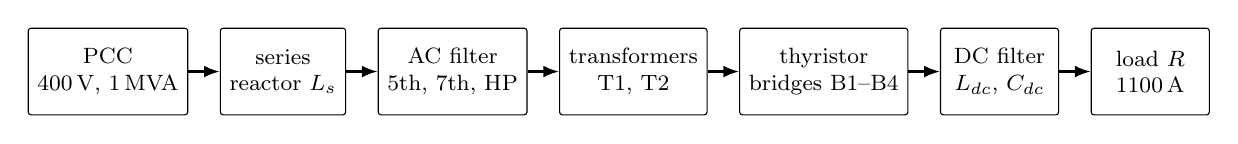
\begin{tikzpicture}[node distance=4mm, every node/.style={font=\small},
  blk/.style={draw, rounded corners=1pt, minimum height=11mm, minimum width=15mm, align=center, font=\footnotesize},
  arr/.style={-{Latex[length=2mm]}, thick}]
\node[blk] (pcc) {PCC\\400\,V, 1\,MVA};
\node[blk, right=of pcc] (ls) {series\\reactor $L_s$};
\node[blk, right=of ls] (fl) {AC filter\\5th, 7th, HP};
\node[blk, right=of fl] (tr) {transformers\\T1, T2};
\node[blk, right=of tr] (br) {thyristor\\bridges B1--B4};
\node[blk, right=of br] (dc) {DC filter\\$L_{dc}$, $C_{dc}$};
\node[blk, right=of dc] (ld) {load $R$\\1100\,A};
\draw[arr] (pcc) -- (ls); \draw[arr] (ls) -- (fl); \draw[arr] (fl) -- (tr);
\draw[arr] (tr) -- (br); \draw[arr] (br) -- (dc); \draw[arr] (dc) -- (ld);
\end{tikzpicture}
\caption{Power chain. The AC filter is connected on the converter side of the series reactor so that the reactor sits between the filter bus and the grid.}
\label{fig:chain}
\end{figure}

\subsection{Supply}

\begin{itemize}
\item PCC voltage $V_{L} = 400$\,V, 50\,Hz, three-phase; rated power of the connection $P_n = 1$\,MW ($S_n = 1$\,MVA).
\item The PCC is assumed to be fed by a 1\,MVA MV/LV transformer with $u_k = 6$\,\%; the MV grid contribution is neglected, so the short-circuit power at the PCC is $S_{sc} \approx S_n/u_k = 16.7$\,MVA and the network reactance at 400\,V is $X_S = V_L^2/S_{sc} = 9.6$\,m$\Omega$. This value must be checked against the real site; it enters only the harmonic-sharing calculation of Section~\ref{sec:acfilter}.
\item Line voltage tolerance $\pm10$\,\% (EN\,50160). The design assumes that the transformers have a primary off-load tap changer with $\pm2\times2.5$\,\% taps, set once at commissioning to the actual site voltage, so that the converter itself has to cover only $\pm5$\,\%.
\end{itemize}

\subsection{Loads}

All loads are resistive, take 1050\,A (1100\,A rated), and have voltages that are integer multiples of a quantum $V_u = 16.4$\,V (Table~\ref{tab:loads}). Only one load is supplied at a time, so the converter must be reconfigurable rather than sized for the sum (which would be 1.93\,MW). The two reference points 20\,V and 200\,V at 1100\,A are treated as additional cases.

\begin{table}[h]
\centering
\begin{tabular}{lrrrrrrrrrr}
\toprule
$V_{out}$ (V) & 196.8 & 164.0 & 147.6 & 131.2 & 98.4 & 82.0 & 65.6 & 49.2 & 32.8 & 16.4\\
$n = V_{out}/V_u$ & 12 & 10 & 9 & 8 & 6 & 5 & 4 & 3 & 2 & 1\\
number of loads & 4 & 1 & 1 & 1 & 3 & 1 & 2 & 1 & 1 & 1\\
$P$ (kW) at 1050\,A & 206.6 & 172.2 & 155.0 & 137.8 & 103.3 & 86.1 & 68.9 & 51.7 & 34.4 & 17.2\\
\bottomrule
\end{tabular}
\caption{Load cases (all at 1050\,A). Sixteen loads, ten distinct voltages, all multiples of 16.4\,V.}
\label{tab:loads}
\end{table}

\subsection{Targets}
\begin{itemize}
\item Line-side current THD at the PCC $\le 5$\,\% (referred to the fundamental of the converter current, i.e.\ the conservative definition; IEC\,61000-3-12 refers harmonics to the rated current, which is less demanding at partial load).
\item Load voltage ripple $\le 5$\,\% peak-to-peak of $V_{out}$.
\item Reactive power at the PCC small enough that no STATCOM is needed: the target adopted here is $|Q_{PCC}| \le 0.15\,S_n = 150$\,kvar at every operating point, with the converter's own lagging demand never larger than what the AC filter capacitors supply.
\end{itemize}

\section{Six-pulse bridge relations used}
\label{sec:basics}

For a fully-controlled six-pulse bridge fed from a secondary line-to-line voltage $\Ell$ (rms), with smooth DC current $\Id$, firing angle $\alpha$ and relative commutation reactance $\ex$ (transformer plus any line reactor, on the secondary rating), the relations of IEC\,60146-1-1 \cite{iec60146} are
\begin{align}
\Vdo &= \frac{3\sqrt2}{\pi}\,\Ell = 1.35\,\Ell, \label{eq:vd0}\\
V_d &= \Vdo\cos\alpha - \dx - 2V_T, \qquad \dx = \frac{\ex}{2}\,\Vdo\,\frac{\Id}{\Id{}_{,r}}, \label{eq:vd}\\
\cos\alpha - \cos(\alpha+u) &= \frac{2\dx}{\Vdo}\quad\text{(overlap angle $u$)}, \label{eq:overlap}\\
I_2 &= \sqrt{\tfrac23}\,\Id = 0.816\,\Id, \qquad I_{1} = \frac{\sqrt6}{\pi}\Id = 0.78\,\Id, \label{eq:i2}\\
S_1 &= \sqrt3\,\Ell I_1 = \Vdo\Id, \qquad \cos\varphi_1 \simeq \frac{\cos\alpha + \cos(\alpha+u)}{2}, \label{eq:s1}\\
P &= S_1\cos\varphi_1 \simeq V_d\Id, \qquad Q = S_1\sin\varphi_1, \label{eq:pq}
\end{align}
where $V_T \approx 1.3$\,V is the on-state drop of one thyristor and two are always in series. Equation~\eqref{eq:s1} is the key to the reactive-power problem: the fundamental apparent power of a bridge is fixed by its no-load voltage, $S_1 = \Vdo \Id$, regardless of how much DC voltage is actually produced. Whatever is not converted into active power ($\Vdo\Id\cos\alpha$) is drawn as reactive power ($\Vdo\Id\sin\alpha$).

The characteristic line-current harmonics ($h = 6k \pm 1$), including the effect of overlap, are \cite{iec60146,kimbark}
\begin{equation}
\frac{I_h}{I_1} = \frac{1}{h}\,
\frac{\sqrt{A^2 + B^2 - 2AB\cos(2\alpha+u)}}{\cos\alpha - \cos(\alpha+u)},\qquad
A = \frac{\sin\frac{(h-1)u}{2}}{h-1},\quad B = \frac{\sin\frac{(h+1)u}{2}}{h+1},
\label{eq:harm}
\end{equation}
which reduce to $I_h/I_1 = 1/h$ for $u \to 0$ (rectangular current, THD\,$= 31$\,\%); with $u = 10$--$20^\circ$ the THD of a single bridge is 26--29\,\%.

The DC-side voltage harmonics of order $n = 6k$ have rms value \cite{kimbark}
\begin{equation}
\frac{V_n}{\Vdo} = \frac{\sqrt2}{n^2-1}\sqrt{1 + (n^2-1)\sin^2\alpha}
\label{eq:vripple}
\end{equation}
i.e.\ 4.0\,\% of $\Vdo$ for the 6th harmonic at $\alpha = 0$, rising to 24\,\% at $\alpha = 90^\circ$. Ripple therefore grows quickly with the firing angle, which is a second reason (besides reactive power) to keep $\alpha$ low.

\section{The reactive-power problem}
\label{sec:q}

Consider first the obvious solution: one transformer and one bridge sized for the highest voltage. With the margins derived in Section~\ref{sec:headroom} the no-load voltage would be $\Vdo \approx 240$\,V, $\Ell \approx 178$\,V. Table~\ref{tab:baseline} gives the operating point for each load voltage.

\begin{table}[h]
\centering
\begin{tabular}{rrrrrr}
\toprule
$V_{out}$ (V) & $\alpha$ (deg) & $P$ (kW) & $Q$ (kvar) & PF & $I_1$ (A)\\
\midrule
16.4 & 83.4 & 17.2 & 230.1 & 0.07 & 333\\
32.8 & 79.1 & 34.4 & 227.9 & 0.15 & 333\\
65.6 & 70.2 & 68.9 & 219.6 & 0.30 & 333\\
98.4 & 60.8 & 103.3 & 205.2 & 0.45 & 333\\
131.2 & 50.4 & 137.8 & 183.3 & 0.60 & 333\\
164.0 & 38.2 & 172.2 & 150.8 & 0.75 & 333\\
196.8 & 20.7 & 206.6 & 97.5 & 0.90 & 333\\
\bottomrule
\end{tabular}

\caption{Single bridge, $\Vdo = 240$\,V, $\ex = 6$\,\%, 1050\,A. The line current is 333\,A at every operating point, only its phase changes.}
\label{tab:baseline}
\end{table}

Below 100\,V the power factor is under 0.45 and the reactive demand is 200--230\,kvar for at most 100\,kW of load: a quarter of the 1\,MVA connection would be spent on reactive power, and a STATCOM or a large, switched capacitor bank would be unavoidable. Note that reactive power is essentially constant at low voltage: $Q \to \Vdo\Id$ as $\alpha \to 90^\circ$. The only way to reduce it is to reduce the $\Vdo$ that is ``in play'' at each operating point. There are three ways to do that.

\paragraph{Tapped transformer.} An off-load tap changer on the secondary (or primary) lowers $\Vdo$ in steps. With $N_t$ taps in a geometric progression of ratio $r$, the worst-case angle is $\alpha_{max} = \arccos(1/(r\,k_h))$ with $k_h$ the headroom factor, and the worst-case reactive power on the top tap is $\Vdo{}_{,top}\Id\sin\alpha_{max}$. With $r = 2$ and $k_h = 1.1$: $\alpha_{max} = 63^\circ$ and $Q_{max} \approx 0.9\,\Vdo{}_{,top}\Id \approx 210$\,kvar -- hardly better, because the large bridge is still the one regulating. Reaching $Q < 100$\,kvar needs about twelve taps (one per 16.4\,V unit) on an 1100\,A winding, which is a costly and slow selector. A tap changer is nevertheless kept in the design in the mild form of $\pm2\times2.5$\,\% primary taps for site-voltage adjustment.

\paragraph{Series bridges with sequential control.} If the converter is split into $m$ bridges connected in series on the DC side, each fed from its own secondary with no-load voltage $\Vdo{}_{,i}$, the output is $\sum_i \Vdo{}_{,i}\cos\alpha_i$ and the reactive power $\sum_i \Vdo{}_{,i}\sin\alpha_i\,\Id$. For a given output voltage the reactive power is minimised by driving the bridges to the extremes -- all at $\alpha_{min}$ or bypassed -- and letting only one bridge regulate. (Since $\sin\alpha$ is a concave function of $\cos\alpha$, equal angles maximise $Q$ for a given $\sum\cos$, Jensen's inequality; the sequential solution is the opposite extreme.) The reactive power is then bounded by the no-load voltage of the regulating bridge, $Q \lesssim \Vdo{}_{,reg}\Id$ plus the small $\sin\alpha_{min}$ contribution of the full bridges. This is the classical sequence control of series-connected rectifiers used in electrolysis and HVDC plants \cite{kimbark}.

\paragraph{Binary weighting.} Because the load voltages are integer multiples of $V_u = 16.4$\,V, four bridges with no-load voltages in the ratio 1:2:4:8 (i.e.\ $V_u$, $2V_u$, $4V_u$, $8V_u$ plus headroom) reach every integer number of units from 1 to 15 by selecting the bridges corresponding to the binary representation of $n$, with the regulating bridge absorbing only the headroom. Four bridges means two transformers with two secondaries each, exactly the ``$N$ transformers with two secondaries'' scheme. Since all bridges carry the same 1100\,A and see secondary voltages between 15 and 110\,V, a single bridge design (same thyristors, same heatsink, same gate drive) serves all four positions; only the transformers differ.

Figure~\ref{fig:qplot} compares the reactive power of the single-bridge and the 1:2:4:8 series solutions over the whole voltage range (1050\,A). The series solution never exceeds 91\,kvar, and the AC filter of Section~\ref{sec:acfilter} supplies 150\,kvar, so the PCC never sees a lagging reactive demand from the converter.

\begin{figure}[h]
\centering
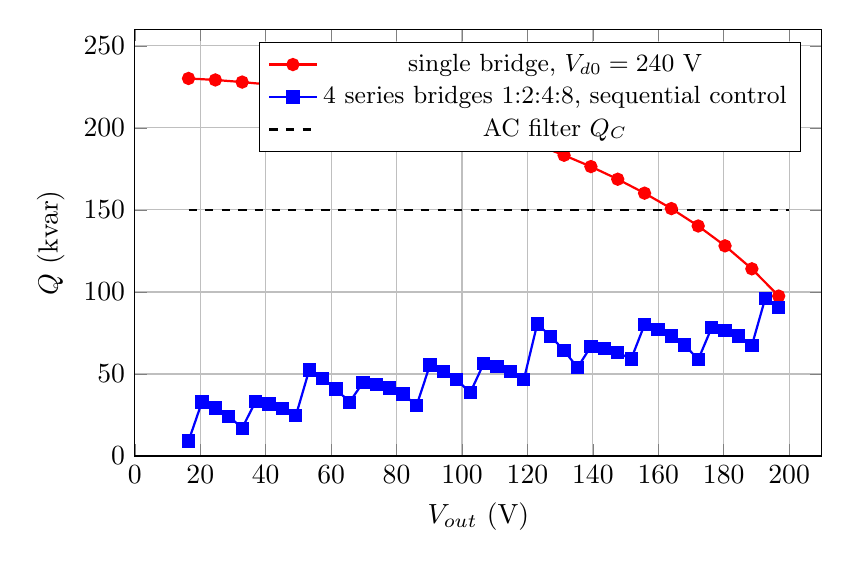
\begin{tikzpicture}
\begin{axis}[width=0.85\textwidth, height=70mm, xlabel={$V_{out}$ (V)}, ylabel={$Q$ (kvar)},
  grid=major, legend pos=north east, legend style={font=\small}, xmin=0, xmax=210, ymin=0, ymax=260]
\addplot[thick,color=red,mark=*] coordinates {(16.4,230.1) (24.6,229.2) (32.8,227.9) (41.0,226.4) (49.2,224.4) (57.4,222.2) (65.6,219.6) (73.8,216.6) (82.0,213.2) (90.2,209.4) (98.4,205.2) (106.6,200.5) (114.8,195.3) (123.0,189.6) (131.2,183.3) (139.4,176.4) (147.6,168.7) (155.8,160.2) (164.0,150.8) (172.2,140.2) (180.4,128.1) (188.6,114.1) (196.8,97.5) };
\addlegendentry{single bridge, $V_{d0}=240$ V}
\addplot[thick,color=blue,mark=square*] coordinates {(16.4,9.1) (20.5,32.9) (24.6,29.2) (28.7,24.3) (32.8,17.0) (36.9,33.3) (41.0,31.8) (45.1,29.1) (49.2,24.5) (53.3,52.5) (57.4,47.3) (61.5,40.9) (65.6,32.8) (69.7,44.7) (73.8,43.6) (77.9,41.5) (82.0,37.8) (86.1,30.7) (90.2,55.5) (94.3,51.7) (98.4,46.5) (102.5,38.6) (106.6,56.2) (110.7,54.5) (114.8,51.6) (118.9,46.6) (123.0,80.5) (127.1,73.0) (131.2,64.3) (135.3,53.9) (139.4,66.8) (143.5,65.5) (147.6,63.1) (151.7,59.1) (155.8,80.1) (159.9,77.1) (164.0,73.1) (168.1,67.6) (172.2,58.8) (176.3,78.2) (180.4,76.3) (184.5,73.1) (188.6,67.4) (192.7,96.2) (196.8,90.6) };
\addlegendentry{4 series bridges 1:2:4:8, sequential control}
\addplot[thick,color=black,dashed] coordinates {(16.4,150) (200,150)};
\addlegendentry{AC filter $Q_C$}

\end{axis}
\end{tikzpicture}
\caption{Reactive power drawn from the AC side at 1050\,A. The saw-tooth of the series solution reflects the bridge combination changing at each multiple of 16.4\,V.}
\label{fig:qplot}
\end{figure}

\section{Series-bridge architecture}
\label{sec:arch}

\begin{figure}[h]
\centering
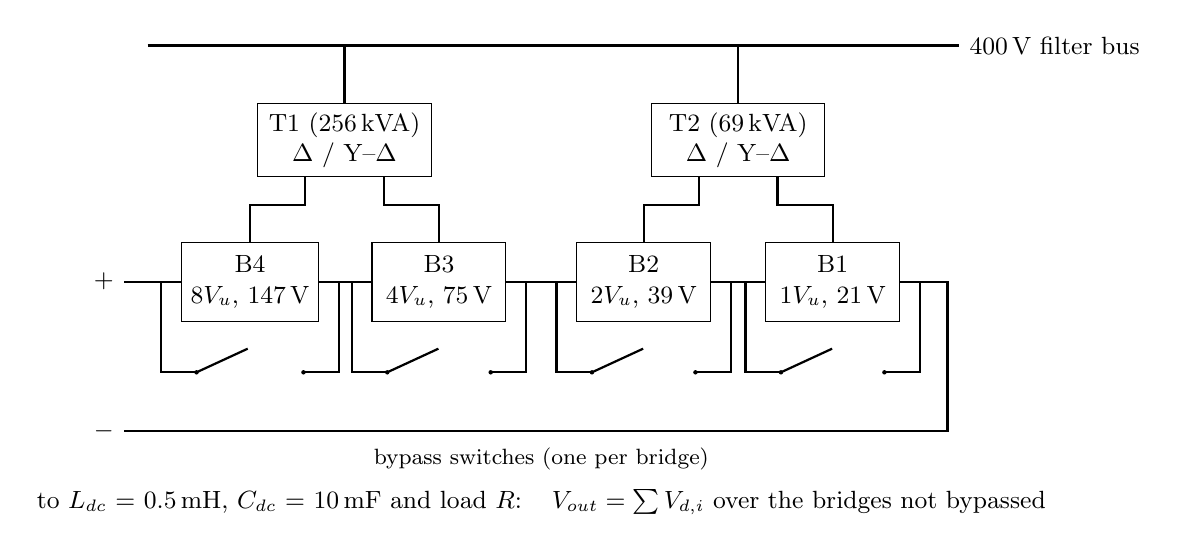
\begin{tikzpicture}[font=\small, every node/.style={align=center},
  tr/.style={draw, minimum width=22mm, minimum height=9mm},
  br/.style={draw, minimum width=17mm, minimum height=10mm}]
% ac bus
\draw[very thick] (-0.5,4.4) -- (9.8,4.4) node[right]{400\,V filter bus};
\node[tr] (t1) at (2.0,3.2) {T1 (256\,kVA)\\$\Delta$ / Y--$\Delta$};
\node[tr] (t2) at (7.0,3.2) {T2 (69\,kVA)\\$\Delta$ / Y--$\Delta$};
\draw[thick] (2.0,4.4) -- (t1.north); \draw[thick] (7.0,4.4) -- (t2.north);
% bridges
\node[br] (b4) at (0.8,1.4) {B4\\$8V_u$, 147\,V};
\node[br] (b3) at (3.2,1.4) {B3\\$4V_u$, 75\,V};
\node[br] (b2) at (5.8,1.4) {B2\\$2V_u$, 39\,V};
\node[br] (b1) at (8.2,1.4) {B1\\$1V_u$, 21\,V};
\draw[thick] ($(t1.south)+(-0.5,0)$) -- ++(0,-0.35) -| (b4.north);
\draw[thick] ($(t1.south)+(0.5,0)$) -- ++(0,-0.35) -| (b3.north);
\draw[thick] ($(t2.south)+(-0.5,0)$) -- ++(0,-0.35) -| (b2.north);
\draw[thick] ($(t2.south)+(0.5,0)$) -- ++(0,-0.35) -| (b1.north);
% series dc string
\draw[thick] (-0.8,1.4) node[left]{$+$} -- (b4.west);
\draw[thick] (b4.east) -- (b3.west);
\draw[thick] (b3.east) -- (b2.west);
\draw[thick] (b2.east) -- (b1.west);
\draw[thick] (b1.east) -- ++(0.6,0) -- ++(0,-1.9) -- (-0.8,-0.5) node[left]{$-$};
% bypass switches: loop under each bridge with an open contact
\foreach \n in {b4,b3,b2,b1}{
  \coordinate (l) at ($(\n.west)+(-0.25,0)$);
  \coordinate (r) at ($(\n.east)+(0.25,0)$);
  \draw[thick] (l) -- ++(0,-1.15) -- ++(0.45,0) coordinate (sl);
  \draw[thick] (r) -- ++(0,-1.15) -- ++(-0.45,0) coordinate (sr);
  \draw[thick] (sl) -- ++(0.65,0.3);
  \fill (sl) circle (0.8pt); \fill (sr) circle (0.8pt);
}
\node[font=\footnotesize] at (4.5,-0.85) {bypass switches (one per bridge)};
\node at (4.5,-1.4) {to $L_{dc}$ = 0.5\,mH, $C_{dc}$ = 10\,mF and load $R$: \; $V_{out} = \sum V_{d,i}$ over the bridges not bypassed};
\end{tikzpicture}
\caption{Four series-connected six-pulse bridges with binary-weighted secondaries and DC bypass switches.}
\label{fig:series}
\end{figure}

\subsection{Operating principle}

For a load of $n$ units the bridges whose weights appear in the binary expansion of $n$ are inserted, the others are bypassed. In fact the dispatch in Table~\ref{tab:cases} was obtained by checking all fifteen combinations and keeping the one with the lowest $Q$ that can deliver the required voltage at $\alpha_{min}$; the binary set is the winner in every case, which confirms the reasoning of Section~\ref{sec:q}. Within the set, the bridges are held at the minimum angle $\alpha_{min} = 10^\circ$ and the smallest bridge of the set regulates; if its range is exhausted (it cannot go below zero average voltage with $\alpha \le 90^\circ$) the next bridge takes over. The current loop acts on the regulating bridge only; the full bridges receive a fixed $\alpha_{min}$ (or, better, a slow voltage-balancing correction). Because the bridges are in series they carry exactly the same current, so there is no current-sharing issue as with parallel bridges, and the current sensor is a single DCCT in the DC string.

$\alpha_{min}$ is kept at $10^\circ$ rather than $0^\circ$ so that the regulating bridge always has authority in both directions (a bridge at $\alpha = 0$ cannot increase its voltage) and to keep the firing point safely after the natural commutation instant under line-voltage distortion.

\subsection{Bypass}

A bridge that is not in use must let the string current through. Two options:

\begin{itemize}
\item \emph{Bypass pair}: two thyristors of the same leg are fired together (e.g.\ T1 and T4), short-circuiting the DC terminals of the bridge through one phase of the secondary. No extra hardware, immediate, and it is the standard HVDC method \cite{kimbark}. The cost is the conduction loss of two thyristors at the full 1100\,A, about $2\times(0.9\,\text{V}\cdot1100\,\text{A} + 0.35\,\text{m}\Omega\cdot1100^2\,\text{A}^2) \approx 2.8$\,kW per bypassed bridge, and a bridge that stays hot and energised.
\item \emph{Mechanical bypass switch} (motorised, 1100\,A DC, off-load operated): zero loss, and the bypassed transformer can be disconnected on the AC side. Since each load has a fixed configuration and the converter is reconfigured off-load between loads, this is the natural choice; the bypass pair remains available as a fast electrical bypass for fault handling (e.g.\ loss of gating on one bridge).
\end{itemize}

The recommended solution is a mechanical bypass on each bridge, interlocked with the AC contactor of the corresponding secondary, with the bypass-pair firing kept in the control firmware.

\subsection{Headroom and no-load voltage of each bridge}
\label{sec:headroom}

A bridge of weight $w$ must deliver $wV_u$ at rated current with the line 5\,\% low, at $\alpha = \alpha_{min}$, with the commutation drop $\dx = (\ex/2)\Vdo$ and two thyristor drops:
\begin{equation}
0.95\,\Vdo\cos\alpha_{min} - \frac{\ex}{2}\Vdo - 2V_T \ge wV_u
\quad\Rightarrow\quad
\Vdo = \frac{wV_u + 2V_T}{0.95\,(\cos\alpha_{min} - \ex/2)} = 1.10\,(wV_u + 2.6\,\text{V}).
\label{eq:vd0i}
\end{equation}
With $\ex = 6$\,\%, $\alpha_{min} = 10^\circ$ and $V_T = 1.3$\,V the headroom factor is $k_h = 1.10$. The thyristor drops are added before the factor because for the 1-unit bridge they are 16\,\% of the output voltage and would otherwise be under-estimated. The resulting bridge and secondary ratings are in Table~\ref{tab:bridges}.

\begin{table}[h]
\centering
\begin{tabular}{lrrrrrr}
\toprule
Bridge & weight & $V_{step}$ (V) & $V_{d0}$ (V) & $E_{2}$ (V) & $I_{2}$ (A) & $S_{2}$ (kVA)\\
\midrule
B1 & 1 & 16.4 & 20.9 & 15.5 & 898 & 24.1\\
B2 & 2 & 32.8 & 38.9 & 28.8 & 898 & 44.8\\
B3 & 4 & 65.6 & 75.0 & 55.5 & 898 & 86.4\\
B4 & 8 & 131.2 & 147.1 & 109.0 & 898 & 169.5\\
\bottomrule
\end{tabular}

\caption{Bridge no-load voltages and secondary ratings ($\Id{}_{,r} = 1100$\,A, $I_2 = 0.816\,\Id$, $S_2 = \sqrt3\Ell I_2 = 1.047\,\Vdo\Id$). Total 325\,kVA.}
\label{tab:bridges}
\end{table}

The maximum output voltage with all four bridges inserted at $\alpha_{min}$ is $0.985\times281.9 - 8.5 - 10.4 \approx 259$\,V at nominal line voltage, i.e.\ the converter also covers loads up to 15 units (246\,V) should they appear.

\section{Operating points}
\label{sec:cases}

Table~\ref{tab:cases} lists, for every load case, the bridge set, the firing angles (regulating bridge first), the active and reactive power, the displacement factor, the fundamental line current referred to 400\,V, the THD of the converter current before the filter (arithmetic sum of the bridge spectra, Eq.~\eqref{eq:harm}, which is conservative because it ignores the partial 5th/7th cancellation between the Y and $\Delta$ secondaries of the same transformer) and the THD at the PCC after the filter of Section~\ref{sec:acfilter}. Values are at nominal line voltage; at $+5$\,\% line the regulating angle increases by 5--10$^\circ$ and $Q$ by roughly 10\,\%.

\begin{table}[h]
\centering
\small
\begin{tabular}{rrrlrrrrrrr}
\toprule
$V_{out}$ & $I_{out}$ & $n$ & bridges & $\alpha$ & $P$ & $Q$ & PF & $I_1$ & THD$_{conv}$ & THD$_{PCC}$\\
(V) & (A) & & (units) & (deg) & (kW) & (kvar) & & (A) & (\%) & (\%)\\
\midrule
196.8 & 1050 & 12 & 4+8 & 32/10 & 206.6 & 90.6 & 0.92 & 337 & 26.3 & 3.7\\
196.8 & 1050 & 12 & 4+8 & 32/10 & 206.6 & 90.6 & 0.92 & 337 & 26.3 & 3.7\\
196.8 & 1050 & 12 & 4+8 & 32/10 & 206.6 & 90.6 & 0.92 & 337 & 26.3 & 3.7\\
147.6 & 1050 & 9 & 1+8 & 53/10 & 155.0 & 63.1 & 0.93 & 255 & 25.8 & 3.5\\
196.8 & 1050 & 12 & 4+8 & 32/10 & 206.6 & 90.6 & 0.92 & 337 & 26.3 & 3.7\\
164.0 & 1050 & 10 & 2+8 & 40/10 & 172.2 & 73.1 & 0.92 & 282 & 26.0 & 3.6\\
131.2 & 1050 & 8 & 8 & 20 & 137.8 & 64.3 & 0.91 & 223 & 27.2 & 3.9\\
98.4 & 1050 & 6 & 2+4 & 32/10 & 103.3 & 46.5 & 0.91 & 173 & 26.3 & 3.7\\
98.4 & 1050 & 6 & 2+4 & 32/10 & 103.3 & 46.5 & 0.91 & 173 & 26.3 & 3.7\\
49.2 & 1050 & 3 & 1+2 & 32/10 & 51.7 & 24.5 & 0.90 & 91 & 26.3 & 3.7\\
98.4 & 1050 & 6 & 2+4 & 32/10 & 103.3 & 46.5 & 0.91 & 173 & 26.3 & 3.7\\
82.0 & 1050 & 5 & 1+4 & 40/10 & 86.1 & 37.8 & 0.92 & 145 & 26.0 & 3.6\\
65.6 & 1050 & 4 & 4 & 20 & 68.9 & 32.8 & 0.90 & 114 & 27.2 & 3.9\\
65.6 & 1050 & 4 & 4 & 20 & 68.9 & 32.8 & 0.90 & 114 & 27.2 & 3.9\\
32.8 & 1050 & 2 & 2 & 20 & 34.4 & 17.0 & 0.90 & 59 & 27.2 & 3.9\\
16.4 & 1050 & 1 & 1 & 20 & 17.2 & 9.1 & 0.88 & 32 & 27.2 & 3.9\\
20.0 & 1100 & 2 & 2 & 52 & 22.0 & 34.9 & 0.53 & 62 & 29.0 & 4.4\\
200.0 & 1100 & 13 & 4+8 & 27/10 & 220.0 & 89.8 & 0.93 & 353 & 26.0 & 3.6\\
\bottomrule
\end{tabular}

\caption{Operating points. $\ex = 6$\,\%, $\alpha_{min} = 10^\circ$, $V_T = 1.3$\,V. The 20\,V reference case uses the 2-unit bridge at $52^\circ$ because 20\,V exceeds what the 1-unit bridge can deliver; its 35\,kvar are nevertheless negligible in absolute terms.}
\label{tab:cases}
\end{table}

Three observations:
\begin{itemize}
\item The reactive demand is at most 91\,kvar (12-unit loads, 207\,kW), i.e.\ the displacement factor never falls below 0.88 except at 20\,V, where the absolute value (35\,kvar) is what matters and is small.
\item The 20\,V and 200\,V reference points are covered with the same hardware. The 12-unit and 13-unit (200\,V) loads both use B3+B4; the difference is absorbed by B3.
\item The regulating bridge is always a small one, so the ripple injected on the DC side by the retarded bridge is small in absolute volts (Section~\ref{sec:dcfilter}).
\end{itemize}

\section{Transformers}
\label{sec:transformers}

Two three-phase transformers, each with a 400\,V delta primary and two secondaries, one star and one delta, giving a 30$^\circ$ phase displacement between the two bridges of the same transformer:

\begin{itemize}
\item \textbf{T1}: secondaries for B4 ($8V_u$, 109\,V, 898\,A, 170\,kVA) and B3 ($4V_u$, 55.5\,V, 898\,A, 86\,kVA); rating 256\,kVA. Carries the bulk of the power; B3 and B4 are used together on the four 196.8\,V loads and on the 200\,V reference case.
\item \textbf{T2}: secondaries for B2 ($2V_u$, 28.8\,V, 898\,A, 45\,kVA) and B1 ($1V_u$, 15.5\,V, 898\,A, 24\,kVA); rating 69\,kVA.
\end{itemize}

Design data common to both:

\begin{itemize}
\item Primary: 400\,V delta, $\pm2\times2.5$\,\% off-load taps. The delta primary also blocks triplen harmonics and, with the star/delta pair of secondaries, gives 12-pulse-like cancellation of the 5th and 7th harmonics in the primary current whenever the two bridges operate at similar angles; this is a bonus not credited in the filter design.
\item Relative commutation reactance seen by each bridge $\ex = 6$\,\% on the secondary rating, including any secondary-side reactor. Both the voltage regulation ($\dx = \ex/2 = 3$\,\% of $\Vdo$) and the harmonic calculation assume this value, so it should be specified as a range (5--7\,\%) rather than a minimum. The mutual reactance between the two secondaries of a transformer must be specified as well, because it determines how the commutation notches of one bridge appear on the other; the IEC\,60146-1-1 short-circuit test of each secondary with the other open and with the other short-circuited gives the two figures.
\item The secondary currents are the six-pulse bridge currents of Eq.~\eqref{eq:i2}, rms $0.816\,\Id$, with harmonic content per Eq.~\eqref{eq:harm}; the harmonic loss factor for winding eddy losses to be declared according to IEC\,61378-1 \cite{iec61378}, $F_{HL} = \sum_h (I_h/I_1)^2 h^2$ up to the 49th, is about 5 for the 6-pulse spectrum at $\alpha_{min}$ with $u \approx 12^\circ$ and reaches 6--7 for the regulating bridge at $50^\circ$; the eddy-loss share of the load losses must be multiplied by this factor. A converter-duty (rectifier) transformer per IEC\,61378-1 is the appropriate specification, not a distribution transformer.
\item Very low secondary voltages (15.5\,V at 898\,A for B1) are normal for electrolysis and magnet-supply transformers but call for foil or bar windings and a careful busbar layout; B1 and B2 could alternatively be built with a single secondary and a centre tap, but the two-secondary solution keeps all bridges identical.
\item Rated voltage of the windings: nominal $+5$\,\% line $+4.6$\,\% bus rise at light load from the filter capacitors through the series reactor (Section~\ref{sec:acfilter}) $\rightarrow$ the core should not saturate at 1.10\,$V_n$; a flux density of 1.5\,T at nominal is a reasonable choice.
\item Inrush: the two transformers are energised separately, T1 (256\,kVA) is the one that matters; a pre-insertion resistor or point-on-wave closing is optional at this size.
\end{itemize}

\section{Thyristor bridges}
\label{sec:bridges}

One bridge design for the four positions: six-pulse, fully controlled, 1100\,A DC continuous, secondary voltage up to 109\,V rms.

\begin{itemize}
\item Currents per device: average $\Id/3 = 367$\,A, rms $\Id/\sqrt3 = 635$\,A, form factor 1.73. With a typical 1600\,V capsule thyristor of $V_{T0} = 0.9$\,V and $r_T = 0.35$\,m$\Omega$ the conduction loss is $0.9\cdot367 + 0.35\cdot10^{-3}\cdot635^2 \approx 470$\,W per device, 2.8\,kW per bridge, 5.6\,kW for the two bridges active on a 12-unit load. Water cooling is convenient but not mandatory; forced air with $R_{th,ca} \approx 0.05$\,K/W per device is feasible.
\item Voltage class: the repetitive peak voltage across a blocking device is $\sqrt2\,\Ell \le 154$\,V; a 1200--1600\,V class is chosen not for the steady state but for switching surges of the transformer, for the commutation overshoot and for the energy of the RC snubber and MOV clamp (see the companion notes on bridge snubbers \cite{snubber}). The low blocking voltage means that the thyristor current rating, not the voltage, is what fixes the device size: an $I_{T(AV)M} \ge 600$--800\,A capsule (or two smaller modules in parallel per position, sharing checked) is the target.
\item Gate drive: the 10$^\circ$ minimum angle and the low secondary voltages require a firm gate pulse train (long pulses, or picket-fence until the current is established), because at $\alpha_{min}$ and low $\Ell$ the anode voltage at the firing instant is only a few volts. Pulse transformers with a $\ge 1$\,A pulse and $di/dt \ge 1$\,A/$\mu$s are recommended.
\item Protection: semiconductor fuses in the AC legs, $I^2t$ coordinated with the thyristor $I^2t$; the 10\,\% series reactor and the transformer reactance limit the prospective fault current at a secondary to about $I_{2,r}/(\ex + 0.10\,S_2/S_{conv})$ -- 9 times rated for B4, 15 times for B1.
\item Bypass: mechanical bypass switch on the DC terminals plus bypass-pair firing capability (Section~\ref{sec:arch}).
\end{itemize}

\section{AC harmonic filter}
\label{sec:acfilter}

\subsection{Why a plain LC low-pass does not work}

A series reactor with a shunt capacitor bank at the converter bus attenuates the harmonic $h$ by $1/[(h/h_r)^2 - 1]$, where $h_r$ is the resonance order of the LC. To attenuate the 5th harmonic by a factor 5 one needs $h_r \approx 2$, which with a 10\,\% reactor implies a capacitor bank of $1/(h_r^2\cdot0.10) = 2.5$\,p.u.\ on the converter base, i.e.\ 800\,kvar. The tuned-filter approach is far cheaper: each branch presents a very low impedance at its tuning frequency, so the converter harmonics are absorbed there instead of flowing into the grid, and the branches supply useful fundamental reactive power.

\subsection{Topology and sharing}

The filter consists of three shunt branches on the 400\,V converter bus: a single-tuned 5th ($h_t = 4.85$), a single-tuned 7th ($h_t = 6.8$) and a second-order damped high-pass tuned at $h_t = 11$ with quality factor 2. A series reactor $L_s$ between this bus and the PCC increases the grid-side impedance seen by the harmonics and hence the share absorbed by the filter. The harmonic current that reaches the PCC is
\begin{equation}
\frac{I_{h,PCC}}{I_{h,conv}} = \left|\frac{Z_F(h)}{Z_F(h) + jh(X_S + X_s)}\right|,
\label{eq:share}
\end{equation}
with $Z_F(h)$ the parallel of the three branches. The converter behaves as a harmonic current source because its own transformer reactance is in series with the source.

\subsection{Sizing}

The series reactor is set at 10\,\% on the converter base ($S_{conv} = 325$\,kVA, $I_{base} = 469$\,A): $X_s = 0.10\cdot400^2/325\,000 = 49$\,m$\Omega$, $L_s = 157$\,$\mu$H. Its continuous current is the vector sum of the converter fundamental (at most 353\,A) and the filter current (216\,A capacitive) plus the residual harmonics: a 400\,A / 160\,$\mu$H iron-core reactor.

The branch sizes were chosen by iteration on the worst operating point (Table~\ref{tab:cases}) to give THD$_{PCC} \le 4.5$\,\% with some margin:

\begin{table}[h]
\centering
\begin{tabular}{lrrrrrr}
\toprule
Branch & $Q_C$ (kvar) & $h_t$ & $f_t$ (Hz) & $C$ ($\mu$F) & $L$ ($\mu$H) & $R$ ($\Omega$)\\
\midrule
5th & 75 & 4.85 & 242 & 1492 & 289 & --\\
7th & 40 & 6.80 & 340 & 796 & 275 & --\\
HP & 35 & 11.00 & 550 & 696 & 120 & 0.83\\
\bottomrule
\end{tabular}

\caption{AC filter branches (per three-phase bank, star-equivalent values at 400\,V). $L = X_C/(h_t^2\omega)$, $C = 1/(\omega X_C)$, $X_C = V_L^2/Q_C$; the high-pass damping resistor is $R = 2\sqrt{L/C}$.}
\label{tab:filter}
\end{table}

\begin{table}[h]
\centering
\small
\begin{tabular}{lrrrrrrrrrr}
\toprule
$h$ & 5 & 7 & 11 & 13 & 17 & 19 & 23 & 25 & 35 & 37\\
\midrule
$|Z_F|$ (m$\Omega$) & 31.7 & 35.1 & 202.9 & 188.6 & 260.3 & 298.6 & 368.2 & 399.1 & 521.6 & 540.7\\
$|Z_S+Z_{ser}|$ (m$\Omega$) & 294.3 & 412.0 & 647.5 & 765.2 & 1000.6 & 1118.4 & 1353.8 & 1471.5 & 2060.2 & 2177.9\\
$I_{h,PCC}/I_{h,conv}$ & 0.098 & 0.079 & 0.290 & 0.217 & 0.217 & 0.221 & 0.224 & 0.224 & 0.214 & 0.211\\
\bottomrule
\end{tabular}

\caption{Filter impedance, grid-side impedance and resulting sharing factor, Eq.~\eqref{eq:share}, for the characteristic harmonics.}
\label{tab:share}
\end{table}

\begin{table}[h]
\centering
\begin{tabular}{lrrrrrrrr}
\toprule
$h$ & 5 & 7 & 11 & 13 & 17 & 19 & 23 & 25\\
\midrule
$I_h/I_1$ converter (\%) & 19.9 & 14.1 & 8.8 & 7.4 & 5.5 & 4.8 & 3.8 & 3.5\\
$I_h/I_1$ at PCC (\%) & 1.94 & 1.12 & 2.57 & 1.61 & 1.20 & 1.07 & 0.86 & 0.78\\
\bottomrule
\end{tabular}

\caption{Worst-case spectrum (20\,V / 1100\,A, bridge B2 at $52^\circ$): converter current before the filter and current at the PCC. THD 29.0\,\% $\rightarrow$ 4.4\,\%.}
\label{tab:spectrum}
\end{table}

The resulting THD at the PCC is between 3.5 and 4.4\,\% over all cases (last column of Table~\ref{tab:cases}). The 11th harmonic is now the largest single component at the PCC; if a lower value is needed, the high-pass branch should be enlarged before the 5th.

Checks:
\begin{itemize}
\item \emph{Parallel resonance} between the filter capacitance and the grid-plus-reactor inductance: with the values above it falls at $h \approx 3.4$ (170\,Hz), with a peak impedance of about 8\,$\Omega$ seen from the converter bus; at 150\,Hz the impedance is 0.6\,$\Omega$. No characteristic harmonic exists there, and the small 3rd harmonic from line unbalance (typically $< 1$\,\% of $I_1$, i.e.\ a few amperes) produces a negligible 3rd-harmonic voltage. The resonance must be re-checked with the real $S_{sc}$: a weaker grid moves it down towards the 3rd harmonic, in which case the 5th branch should be detuned to $h_t = 4.7$ or the high-pass converted to a C-type.
\item \emph{Background distortion}: a 3\,\% 5th-harmonic voltage on the grid drives $0.03\cdot231/(5\cdot0.059 + 0.032) \approx 21$\,A into the 5th branch, well within its rating.
\item \emph{Fundamental voltage}: the 150\,kvar flow through the 10\,\% reactor and raise the converter bus by $Q_C X_s/V_L^2 = 4.6$\,\% at no load (accounted for in the transformer voltage rating). Capacitors rated $\ge 480$\,V (525\,V class preferred), with a current rating that includes the tuned-harmonic component (the 5th branch carries essentially the whole converter 5th harmonic, up to 70\,A at 400\,V).
\item \emph{Reactive balance}: the converter demand is 9--91\,kvar lagging, the filter supplies 150\,kvar leading, so the PCC sees between 60 and 140\,kvar \emph{leading}. This is within the $0.15\,S_n$ budget and removes the need for a STATCOM. If the utility contract penalises leading power factor, the 7th and high-pass branches (75\,kvar) can be switched off below 4 units of load with only a marginal THD penalty at those small currents, and the whole filter is switched together with the converter main contactor so that nothing is left connected at standstill.
\end{itemize}

An alternative with 120\,kvar of filter (60/30/30) and a 12\,\% series reactor gives THD$_{PCC} = 4.6$\,\%; the 150\,kvar / 10\,\% combination was preferred for margin and lower bus-voltage rise.

\section{DC filter}
\label{sec:dcfilter}

The 6th-harmonic (300\,Hz) ripple voltage at the output of the series string is the sum of the contributions of the inserted bridges, Eq.~\eqref{eq:vripple}, taken arithmetically (worst case; the star/delta 30$^\circ$ shift actually puts the 6th harmonics of the two bridges of the same transformer in phase opposition). The LC filter loaded by $R = V_{out}/I_{out}$ transfers this ripple to the load with
\begin{equation}
H(j\omega_6) = \frac{1}{1 - \omega_6^2 L_{dc}C_{dc} + j\omega_6 L_{dc}/R}.
\end{equation}
Because the load resistance is very small (15--190\,m$\Omega$) the reactor alone already attenuates strongly ($\omega_6 L_{dc}/R = 2.5$ to 30); the capacitor adds the LC attenuation and is what keeps the ripple within specification at the higher voltages.

Chosen values: $L_{dc} = 0.5$\,mH (1100\,A, stored energy 300\,J) and $C_{dc} = 10$\,mF (electrolytic bank, $\ge 300$\,V), resonance at 71\,Hz, well below 300\,Hz and heavily damped by the load ($\zeta = \tfrac{1}{2R}\sqrt{L/C} \ge 0.6$ at 200\,V, $> 7$ at 20\,V). Table~\ref{tab:dcripple} gives the result for every case: the peak-to-peak load-voltage ripple is at most 2\,\% (target 5\,\%), and the 300\,Hz current ripple in the reactor and bridges stays below 6\,\% peak-to-peak, which validates the smooth-current assumption used for the AC harmonics. The reactor also guarantees continuous conduction at the largest firing angle (20\,V case, $\alpha = 52^\circ$).

\begin{table}[h]
\centering
\small
\begin{tabular}{rrlrrrrr}
\toprule
$V_{out}$ & $I_{out}$ & bridges & $\alpha$ & $V_6$ bridge & $V_6$ load & $\Delta V_{pp}/V_{out}$ & $\Delta I_{pp}/I_{out}$ reactor\\
(V) & (A) & (units) & (deg) & (V rms) & (V rms) & (\%) & (\%)\\
\midrule
196.8 & 1050 & 4+8 & 32/10 & 18.5 & 1.06 & 1.52 & 5.6\\
196.8 & 1050 & 4+8 & 32/10 & 18.5 & 1.06 & 1.52 & 5.6\\
196.8 & 1050 & 4+8 & 32/10 & 18.5 & 1.06 & 1.52 & 5.6\\
147.6 & 1050 & 1+8 & 53/10 & 12.6 & 0.70 & 1.33 & 3.8\\
196.8 & 1050 & 4+8 & 32/10 & 18.5 & 1.06 & 1.52 & 5.6\\
164.0 & 1050 & 2+8 & 40/10 & 14.8 & 0.83 & 1.43 & 4.4\\
131.2 & 1050 & 8 & 20 & 13.6 & 0.74 & 1.59 & 4.1\\
98.4 & 1050 & 2+4 & 32/10 & 9.5 & 0.49 & 1.40 & 2.8\\
98.4 & 1050 & 2+4 & 32/10 & 9.5 & 0.49 & 1.40 & 2.8\\
49.2 & 1050 & 1+2 & 32/10 & 5.0 & 0.19 & 1.10 & 1.5\\
98.4 & 1050 & 2+4 & 32/10 & 9.5 & 0.49 & 1.40 & 2.8\\
82.0 & 1050 & 1+4 & 40/10 & 7.6 & 0.37 & 1.28 & 2.3\\
65.6 & 1050 & 4 & 20 & 6.9 & 0.31 & 1.32 & 2.0\\
65.6 & 1050 & 4 & 20 & 6.9 & 0.31 & 1.32 & 2.0\\
32.8 & 1050 & 2 & 20 & 3.6 & 0.10 & 0.90 & 1.0\\
16.4 & 1050 & 1 & 20 & 1.9 & 0.03 & 0.53 & 0.6\\
20.0 & 1100 & 2 & 52 & 7.5 & 0.14 & 1.96 & 2.1\\
200.0 & 1100 & 4+8 & 27/10 & 17.1 & 0.98 & 1.38 & 4.9\\
\bottomrule
\end{tabular}

\caption{DC-side 6th-harmonic ripple with $L_{dc} = 0.5$\,mH, $C_{dc} = 10$\,mF. $V_6$ bridge is the worst-case sum of the inserted bridges.}
\label{tab:dcripple}
\end{table}

The capacitor ripple current is $\omega_6 C_{dc} V_{6,load} \le 20$\,A rms -- trivial for a 10\,mF bank -- and a smaller bank (2--5\,mF) would still meet the 5\,\% target; 10\,mF was kept for margin against the arithmetic-sum assumption and for load-step damping. If a smaller reactor is desired, $L_{dc} = 0.3$\,mH with $C_{dc} = 10$\,mF gives about 2.7\,\% voltage ripple and 10\,\% reactor current ripple.

\section{Summary of the design}

\begin{table}[h]
\centering
\footnotesize
\begin{tabular}{lp{130mm}}
\toprule
Item & Rating\\
\midrule
PCC & 400\,V, 1\,MVA, $S_{sc} \approx 16.7$\,MVA (to be verified)\\
Series reactor $L_s$ & 157\,$\mu$H (10\,\% on 325\,kVA), 400\,A\\
AC filter & 5th: 75\,kvar, 1492\,$\mu$F, 289\,$\mu$H; 7th: 40\,kvar, 796\,$\mu$F, 275\,$\mu$H;\\
 & HP: 35\,kvar, 696\,$\mu$F, 120\,$\mu$H, 0.83\,$\Omega$; capacitors 525\,V class\\
Transformer T1 & 256\,kVA, 400\,V $\Delta$ $\pm2\times2.5$\,\%, secondaries 109\,V (Y) and 55.5\,V ($\Delta$), 898\,A each, $\ex = 6$\,\%\\
Transformer T2 & 69\,kVA, 400\,V $\Delta$ $\pm2\times2.5$\,\%, secondaries 28.8\,V (Y) and 15.5\,V ($\Delta$), 898\,A each, $\ex = 6$\,\%\\
Bridges B1--B4 & 4 identical six-pulse fully-controlled bridges, 1100\,A, 1600\,V class thyristors $I_{T(AV)} \ge 600$\,A,\\
 & DC bypass switch each, series connected, sequential control with $\alpha_{min} = 10^\circ$\\
DC filter & $L_{dc} = 0.5$\,mH / 1100\,A, $C_{dc} = 10$\,mF / 300\,V\\
Performance & $V_{out}$ 16.4--259\,V at 1100\,A; $Q_{conv} \le 91$\,kvar; $Q_{PCC}$ 60--140\,kvar leading;\\
 & THD$_{PCC} \le 4.4$\,\%; load voltage ripple $\le 2$\,\% pp\\
\bottomrule
\end{tabular}
\caption{Design summary.}
\end{table}

Open points to be settled with the real site data: the short-circuit power at the PCC (filter resonance), the utility's rule on leading reactive power (filter switching), and whether loads other than the sixteen listed may appear (the string covers up to 15 units).

\begin{thebibliography}{9}
\bibitem{iec60146} IEC 60146-1-1, \emph{Semiconductor converters -- General requirements and line commutated converters -- Part 1-1: Specification of basic requirements}.
\bibitem{iec61378} IEC 61378-1, \emph{Converter transformers -- Part 1: Transformers for industrial applications}; IEC 60076-6, \emph{Power transformers -- Part 6: Reactors}.
\bibitem{iec61000} IEC 61000-3-12, \emph{Limits for harmonic currents produced by equipment connected to public low-voltage systems with input current $>16$\,A and $\le 75$\,A per phase}; IEEE Std 519-2022, \emph{Harmonic control in electric power systems}.
\bibitem{kimbark} E.~W. Kimbark, \emph{Direct Current Transmission}, Vol.~1, Wiley, 1971 (converter harmonics, sequence control, bypass pair).
\bibitem{mohan} N.~Mohan, T.~M. Undeland, W.~P. Robbins, \emph{Power Electronics: Converters, Applications and Design}, 3rd ed., Wiley, 2003.
\bibitem{arrillaga} J.~Arrillaga, N.~R. Watson, \emph{Power System Harmonics}, 2nd ed., Wiley, 2003 (tuned and high-pass filter design).
\bibitem{snubber} D.~Bagnara, \emph{Snubber design for diode and thyristor bridges} and \emph{IEC 60146-1-1 line reactor sizing}, internal notes, 2026.
\end{thebibliography}

\end{document}
